\section{3D Rendering Grundlagen}
In den weiterführenden Abschnitten werden Kenntnisse über grundlegende Begriffe und Konzepte des 3D Renderings benötigt.
Deshalb werden diese in diesem Abschnitt erklärt.
Die benötigten Themen wurden in WebGL: up and running \cite[4-9]{parisi2012webgl} passend zu den folgenden Kapiteln gegliedert, deshalb wurde die Struktur dieser Grundlagen an diese angelehnt.

\subsection{3D Koordinatensystem}
Beim rendern von 2D Elementen wird ein einfach 2D Koordinatensystem verwendet, genauso wie man es aus der Mathematik kennt. Dort gibt es eine x- und eine y-Achse durch welche die Koordinaten der einzelnen Punkte beschrieben werden können.
Dabei ist es üblich, dass die x-Achse horizontal liegt und somit bestimmt wie weit Links oder Rechts der Punkt ist. Die y-Achse hingegen bestimmt wie hoch und tief ein Punkt liegt.
Um nun zum 3D Koordinatensystem zu kommen, wird einfach eine dritte Achse hinzugefügt, die z-Achse. Diese steht beim WebGL Koordinatensystem so gesehen aus dem Bildschirm heraus, das heißt,
 negative Werte geben an wie tief ein Punkt im Bildschirm liegt.\cite[4]{parisi2012webgl} In Abbildung~\ref{fig:3DKoordinatensystem} sieht man exemplarisch ein solches 3D Koordinatensystem.
 \begin{figure}
    \centering
    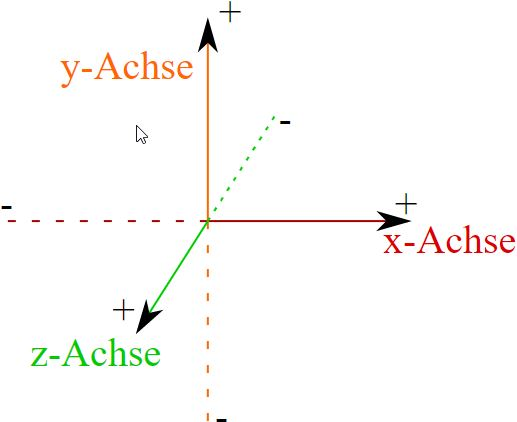
\includegraphics[width=6cm]{3dkoords.jpg}
    \caption{3D Koordinatensystem \cite{PeterStrohm}} \label{fig:3DKoordinatensystem}
    \end{figure}

\subsection{Gittergewebe, Polygone und Eckpunkte}
\subsection{Materialien, Texturen und Lichter}
\subsection{Transformationen und Matrizen}
\subsection{Kamreas, Perspektiven, Ansichtsfenster und Projektionen}
\subsection{Shader}

